% LaTeX Vorlage
%\documentclass[
%  ngerman,		% Sprache
%  a4paper,		% Papierformat
%  11pt,			% Schriftgröße (default 10pt)
%  DIV=12,		% Seiteneinteilung
%  parskip=half  	% Absätze (full,half,false -+*)
%]{scrartcl}
\documentclass{beamer}
%\documentclass[handout]{beamer}

\usepackage[utf8]{inputenc} % UTF-8
\usepackage[ngerman,english,main=english]{babel} % Sprache 
\selectlanguage{english}
\usepackage{amsmath, amssymb}
\usepackage{graphicx} % Grafiken einbinden
%\usepackage[left=2cm,right=2cm,top=2.5cm,bottom=3cm]{geometry}
\usepackage{color} % Farbe
\usepackage{bbm}

\usetheme{Boadilla}
%\usetheme{ AnnArbor | Antibes | Bergen | Berkeley | Berlin | Boadilla | boxes | CambridgeUS | Copenhagen | Darmstadt | default | Dresden | 	Frankfurt | Goettingen |Hannover | Ilmenau | JuanLesPins | Luebeck | Madrid | Malmoe | Marburg | Montpellier | PaloAlto | Pittsburgh | Rochester | Singapore | Szeged | Warsaw }
\usecolortheme{whale}
%\usecolortheme{ albatross | beaver | beetle | crane | default | dolphin | dove | fly | lily | orchid | rose |seagull | seahorse | sidebartab |structure | whale | wolverine }
\usefonttheme{default}
%\usefonttheme{ default | professionalfonts | serif | structurebold | structureitalicserif | structuresmallcapsserif }

% Innere Themen spezifizieren die inneren Elemente wie Kopf-, Fußzeile, Sidebar usw. einer Folie.
\useinnertheme{rectangles}
% \useinnertheme{
% 	circles | default | inmargin |
% 	rectangles | rounded
% }

% Äußere Themen spezifizieren die Grenzen einer Folie und sagen ob und wo die inneren Elemente liegen.
% \useoutertheme{
% 	default | infolines | miniframes |
% 	shadow | sidebar | smoothbars |
% 	smoothtree | split | tree
% }

% Um halbtransparente Overlays auf seinen Folien zu haben, reicht es folgenden Schalter zu setzen:
% \setbeamercovered{transparent}

% Zum Abschalten der kleinen Navigationsleiste am unteren Rand reicht folgende Zeile aus:
% \beamertemplatenavigationsymbolsempty

% Seitenzahlen in Fußzeile einfügen
\setbeamertemplate{footline}[frame number]


% Um die Metainfomationen zu setzen die unter anderem für die Titelseite verwendet werden, kann man sich folgender Befehle bedienen:
\title{Next-to-Leading Order QCD Corrections to Inclusive Heavy-Flavor Production in Polarized Deep-Inelastic Scattering} % Titel des Vortrages
%\subject{Higgs-Mechanismus} % Setzt Thema in den PDF-Dokument-Eigenschaften
%\subtitle[Masseerzeugung]{oder warum das Photon auf Diät gesetzt wurde} % Untertitel

\author[F. Hekhorn]{Felix Hekhorn} % Autor festlegen
\institute{Institute for Theoretical Physics, University of T\"ubingen}
% \institute[IfI -- HU Berlin]{Institut für Informatik\\ Humboldt-Universität zu Berlin}
%     Angabe des Institutes
%\date[13.12.12]{13. Dezember 2012} % Datum der Präsentation, alternativ kann mittels \date{\today} auch das aktuelle Datum eingetragen werden.
% \logo{\pgfimage[width=2cm,height=2cm]{hulogo}}
%     Die Datei hulogo.pdf (bzw. hulogo.png, hulogo.jpg, hulogo.mps bei Verwendung von pdftex als Backend) als Logo auf allen Folien, hier mithilfe des Paketes pgf.
% \titlegraphic{\includegraphics[width=2cm,height=2cm]{hulogo}}
%     Die Datei hulogo.pdf (bzw. analog wie bei \logo auch entsprechendes Format) als Logo nur auf der Titelseite unter Verwendung des Paketes graphicx.

\usepackage{pgfpages}
%\pgfpagesuselayout{resize to}[a4paper,border shrink=5mm,landscape]
%\pgfpagesuselayout{2 on 1}[a4paper,border shrink=5mm]
%\pgfpagesuselayout{4 on 1}[a4paper,border shrink=5mm,landscape]
%\pgfpagesuselayout{8 on 1}[a4paper,border shrink=5mm]
%\pgfpagesuselayout{16 on 1}[a4paper,border shrink=5mm,landscape]

%\usepackage{pdflscape}

\usepackage{slashed}

\usepackage{wrapfig}
\usepackage{graphicx}
\usepackage{pdflscape}
\usepackage{ulem}
\usepackage{url}
\usepackage{caption}
\usepackage{subcaption}
\usepackage{array}
\usepackage{multirow}
\usepackage{listings}
\usepackage{placeins}
\usepackage{csquotes}

\usepackage{siunitx} % SI Einheiten
\usepackage[version=3]{mhchem}
%\sisetup{
%	exponent-product = \!\cdot\!,
%	output-product = \cdot,
%	list-final-separator =  { und } ,
%	list-pair-separator = { und } ,
%	range-phrase = { bis },
%	output-decimal-marker = {,},
%	separate-uncertainty = true,
%	group-digits = false
%}

%\usepackage{simplewick}
%\usepackage{feynmf}
\usepackage{slashed}
\usepackage{hepnames}

\usepackage{url}
\usepackage{hyperref}
%\hypersetup{colorlinks=false}
\usepackage{tabularx}

\providecommand{\abs}[1]{\left|#1\right|}
\providecommand{\VektorV}[3]{
\!\left(\!\!
\begin{array}{c}
#1 \\ #2 \\ #3
\end{array}\!\!
\right)\!
}

\providecommand{\Det}[9]{
	\begin{vmatrix}
	    #1 & #2 & #3 \\
	    #4 & #5 & #6 \\
	    #7 & #8 & #9 \\	    
	\end{vmatrix}
}

\DeclareMathOperator{\Grad}{\text{grad}}
\DeclareMathOperator{\Div}{\text{div}}
\DeclareMathOperator{\Rot}{\text{rot}}
\DeclareMathOperator{\tr}{\text{tr}}

\DeclareMathOperator{\acos}{\text{arccos}}
\DeclareMathOperator{\asin}{\text{arcsin}}
\DeclareMathOperator{\atanh}{\text{artanh}}
\DeclareMathOperator{\x}{\times}
\DeclareMathOperator{\cdt}{\!\cdot\!}
\DeclareMathOperator{\del}{\partial}
\DeclareMathOperator{\EqualClaim}{\stackrel{!}{=}}
\DeclareMathOperator{\equivals}{\mathrel{\widehat{=}}}
\providecommand{\Nabla}[0]{\vec\nabla}
\providecommand{\ex}[1]{e^{#1}}
\providecommand{\EE}[1]{\cdot 10^{#1}}
\providecommand{\FT}[1]{\mathcal{FT}\left[#1\right]}
\providecommand{\Mel}[1]{\mathcal{M}\left[#1\right]}
\providecommand{\invMel}[1]{\mathcal{M}^{-1}\left[#1\right]}

\providecommand{\dt}[0]{\Derive t}
\providecommand{\dx}[0]{\Derive x}
\providecommand{\Derive}[1]{\DeriveN{#1}{}}
\providecommand{\DeriveN}[2]{\DeriveNF {#1}{#2}{}}
\providecommand{\DeriveF}[2]{\DeriveNF {#1}{}{#2}}
\providecommand{\DeriveNF}[3]{\frac {d^{#2}#3} {d #1^{#2}}}
\providecommand{\dtP}[0]{\DeriveP t}
\providecommand{\dxP}[0]{\DeriveP x}
\providecommand{\DeriveP}[1]{\DerivePN{#1}{}}
\providecommand{\DerivePF}[2]{\DerivePNF {#1} {} {#2}}
\providecommand{\DerivePN}[2]{\DerivePNF {#1} {#2} {} }
\providecommand{\DerivePNF}[3]{\frac {\partial^{#2}#3} {\partial #1^{#2}}}
\providecommand{\DerivePMF}[3]{\frac {\partial^{2}#3} {\partial #1 \partial #2}}
\providecommand{\e}[1]{\hat{e}_{#1}}
\providecommand{\pFq}[2]{{}_{#1}F_{#2}}

\providecommand{\bra}[1]{\langle#1\rvert}
\providecommand{\ket}[1]{\lvert#1\rangle}
\providecommand{\bracket}[2]{\langle#1\vert#2\rangle}
\providecommand{\normOrd}[1]{\,:\!#1\!:\,}
\providecommand{\wContr}[3]{\contraction{}{#1}{#2}{#3}#1#2#3}

\DeclareMathOperator{\und}{\text{UND}}
\DeclareMathOperator{\oder}{\text{ODER}}

\DeclareMathOperator{\Md}{\mathcal M}
\DeclareMathOperator{\Ld}{\mathcal L}
\DeclareMathOperator{\Hd}{\mathcal H}
\DeclareMathOperator{\Nd}{\hat {\mathcal N}}
\DeclareMathOperator{\To}{\hat {\mathcal T}}

\DeclareMathOperator{\ijI}{\mathit{ij},\mathbf{I}}
\DeclareMathOperator{\MSbar}{\overline{\text{MS}}}


\DeclareRobustCommand{\PQ}{\HepGenParticle{Q}{}{}\xspace} % quark
\DeclareRobustCommand{\PaQ}{\HepGenAntiParticle{Q}{}{}\xspace} % anti-quark


\begin{document}

\frame{ \titlepage }
\frame{
	\frametitle{Outline}
	\tableofcontents
}

\section{Introduction}

\begin{frame}{Introduction - Heavy Quarks (HQ)}
\begin{itemize}
\item Heavy Quarks (HQ): $\Pcharm (m_{\Pcharm}=\SI{1.5}{\GeV})$, $\Pbottom (m_{\Pbottom}=\SI{4.75}{\GeV})$, $\Ptop (m_{\Ptop}=\SI{175}{\GeV})$
\item EIC will reach region with HQ relevant to structure functions
\item compare unpolarized case @HERA: at small $x$ $\sim 30\%$ charm contributions
\item<2-> measure $\Delta g$ as dominated by PGF
\item<2-> first NLO computation of polarized process
\end{itemize}
\begin{itemize}
\item<3-> need improved charm tagging
\item<3-> full inclusive cross section is complicated to reconstruct
\item<3-> no hadronization here
\end{itemize}
\end{frame}

\begin{frame}{Introduction - Heavy Quarks (HQ)}
\newcolumntype{w}{>{\centering\arraybackslash} m{.7\linewidth} }
\newcolumntype{i}{>{\centering\arraybackslash} m{.3\linewidth} }
\begin{tabular}{wi}
\begin{itemize}
%\setlength{\itemindent}{-1em}
\item scale of hard process is in a pertubative regime $m>\Lambda_{QCD}$
\item finite mass $m$ ensures full inclusive cross sections
\item<2-> full $m^2$ dependence makes computations complicated: phase space + matrix elements
\item<2-> 2-scale problem: $\ln\left(\frac{s-4m^2}{4m^2}\right)$ and/or $\ln(Q^2/m^2)$
\item<2-> keep analytic expressions
\end{itemize}
&
\only<beamer>{\includegraphics[width=.27\textwidth]{img/c2}}
\end{tabular}
\end{frame}

\begin{frame}{Introduction - DIS Setup}
\[\Pem(l_1)+h(p) \to \Pem(l_2) + \PaQ(p_2) + X[\PQ]\]
\newcolumntype{w}{>{\centering\arraybackslash} m{.74\linewidth} }
\newcolumntype{i}{>{\centering\arraybackslash} m{.26\linewidth} }
\hspace{-.5cm}\begin{tabular}{iw}
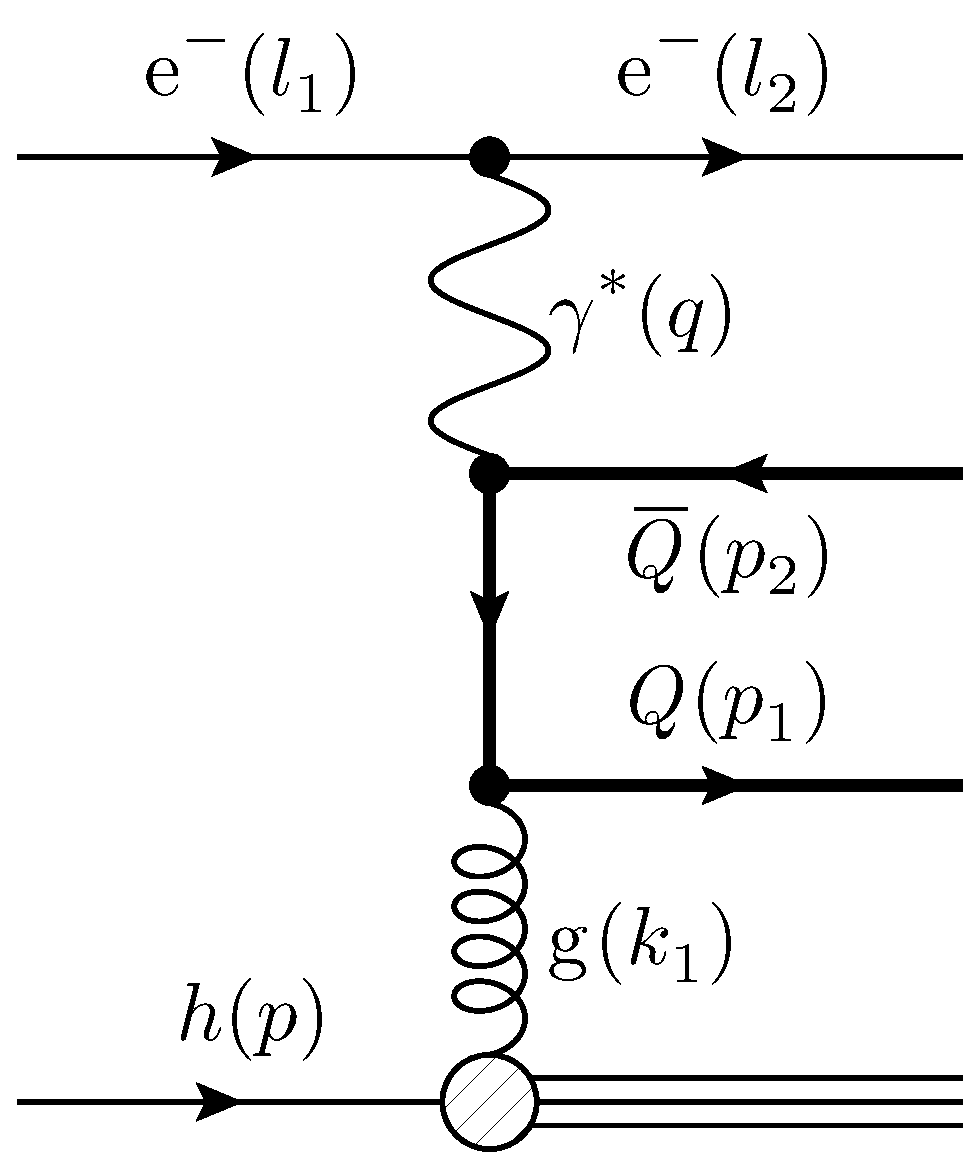
\includegraphics[width=.25\textwidth]{img/DIS.eps} &
\begin{itemize}
\item $S_h = (p+l_1)^2 = x\,y\,Q^2,\,x,\,y,$\\
$Q^2 = -q^2 = - (l_1-l_2)^2 \ll M_Z^2$
\item unpolarized cross section:\\
$\frac{d^2\sigma}{dx dy} = \frac{2\pi \alpha^2}{x y Q^2}\left(Y_+F_2(x,Q^2) - y^2F_L(x,Q^2)\right)$\\
$2xF_1(x,Q^2) = F_2(x,Q^2) - F_L(x,Q^2)$
\item polarized cross section:\\
$\frac{d^2\Delta\sigma}{dx dy} = \frac{4\pi \alpha^2}{x y Q^2}Y_-\cdot 2xg_1(x,Q^2)$
\item with $Y_\pm = 1 \pm (1-y)^2$
\item $[k=T]\to 2xF_1$, $[k=L]\to F_L$ and $[k=P]\to 2xg_1$
\end{itemize}
\end{tabular}
\end{frame}

%%%
\iffalse
\begin{frame}{Introduction - Experimental Setups}
\begin{center}
\newcolumntype{C}{>{\centering\arraybackslash} m{3.6cm} } 
\begin{tabular}{C|C|C}
\Pelectron-\APelectron-annihilation (SIA) & deep inelastic scattering (DIS) & Drell-Yan process (DY)\\
%SIA & DIS & DY\\
\hline
\vspace{3pt}
$\Pelectron+\APelectron \to \PaQ + X[\PQ]$ &
\vspace{3pt}
$\Pl+h \to \Pl' + \PaQ + X[\PQ]$ &
\vspace{3pt}
$h + h' \to \PaQ + X[\PQ]$ \\
\hline
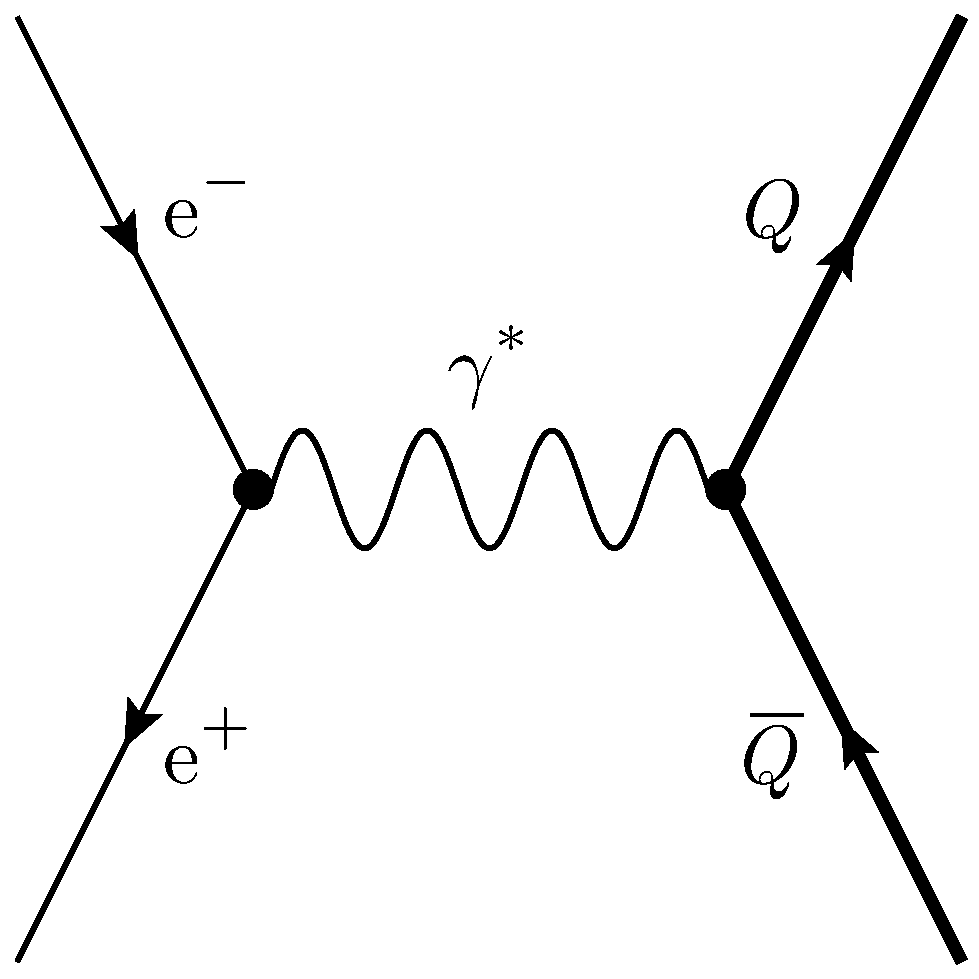
\includegraphics[width=.25\textwidth]{img/SIA.eps} & 
\vspace{.2cm}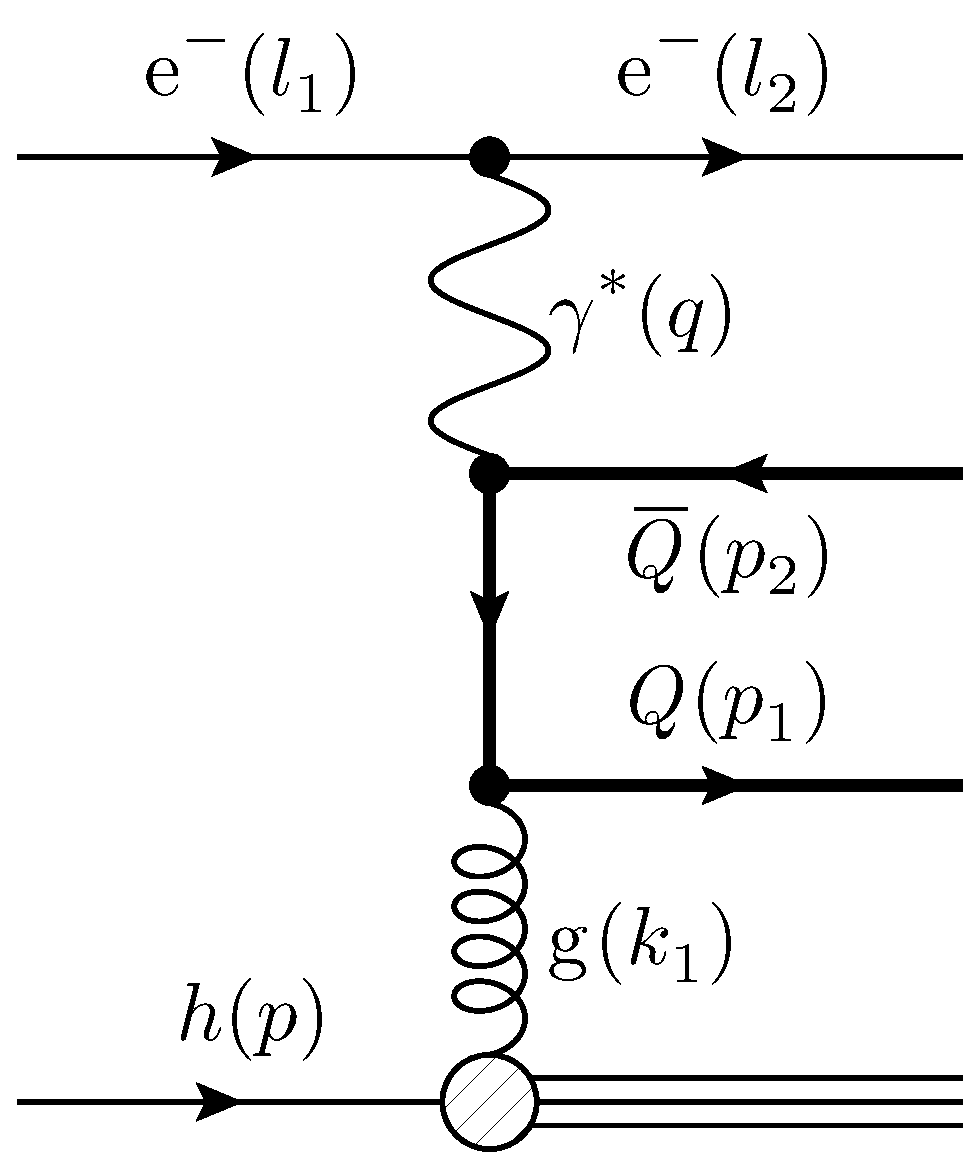
\includegraphics[width=.25\textwidth]{img/DIS.eps} & 
\vspace{.2cm}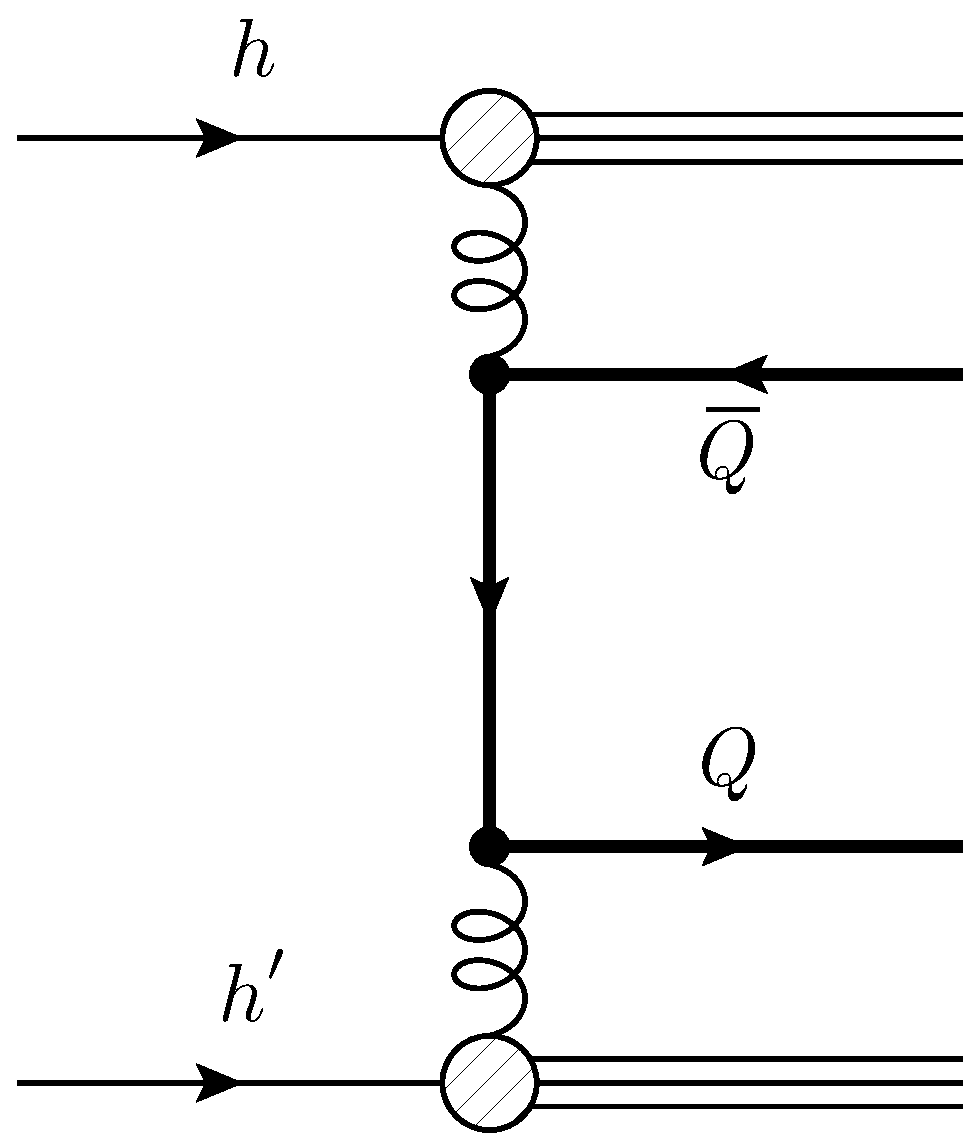
\includegraphics[width=.25\textwidth]{img/DY.eps} \\
\hline
LEP, ILC & \vspace{2pt} HERA, COMPASS, EIC & Tevatron, LHC\\
\hline
gluon & factorization & top, Higgs
\end{tabular}
\end{center}
\end{frame}

\begin{frame}{Introduction - Structure Functions}
\begin{align}
&\text{cross section (xs):}&\frac{d^2\sigma}{dx dy} &= \frac{2\pi y \alpha^2}{Q^4} L^{\mu\nu} W_{\mu\nu}\\
&\text{hadronic tensor:}&W_{\mu\nu} &= \left(-g_{\mu\nu} + \frac{q_\mu q_\nu}{q^2}\right) F_1(x,Q^2) + \frac{P_\mu P_\nu}{P\cdot q} F_2(x,Q^2) \nonumber\\
&& & \hspace{20pt} + i \epsilon_{\mu\nu\alpha\beta} \frac{q^{\alpha}S^{\beta}}{P\cdot q} g_1(x,Q^2)\\
&&F_L(x,Q^2) &= F_2(x,Q^2) - 2xF_1(x,Q^2)\\
&\text{unpolarized xs:}&\frac{d^2\sigma}{dx dy} &= \frac{2\pi \alpha^2}{x y Q^2}\left(Y_+F_2(x,Q^2) - y^2F_L(x,Q^2)\right)\\
&\text{polarized xs:}&\frac{d^2\Delta\sigma}{dx dy} &= \frac{4\pi \alpha^2}{x y Q^2}Y_-\cdot 2xg_1(x,Q^2)\\
&&Y_\pm &= 1 \pm (1-y)^2
\end{align}
\end{frame}
\fi
%%%


\section{Computation Review}
\begin{frame}{Computation Review}
\begin{itemize}
\item use factorisation theorem: PDF and $s=\xi S_h$
\item PGF: $\Pg(k_1) + \Pggx(q) \to \PaQ(p_2) + \PQ(p_1)$
\item three massive particles: $m^2>0,q^2=-Q^2<0$
\item<2-> compute 2-to-3-phase space: e.g. $dPS_3 \sim dt_1du_1d\Omega_nd\hat{\mathcal{I}}$ \iRef{Laenen, Bojak}
\item<2-> diagrams: %
\raisebox{-.4\height}{\includegraphics[height=.15\textheight]{img/nlo-g-4}} +%
\raisebox{-.4\height}{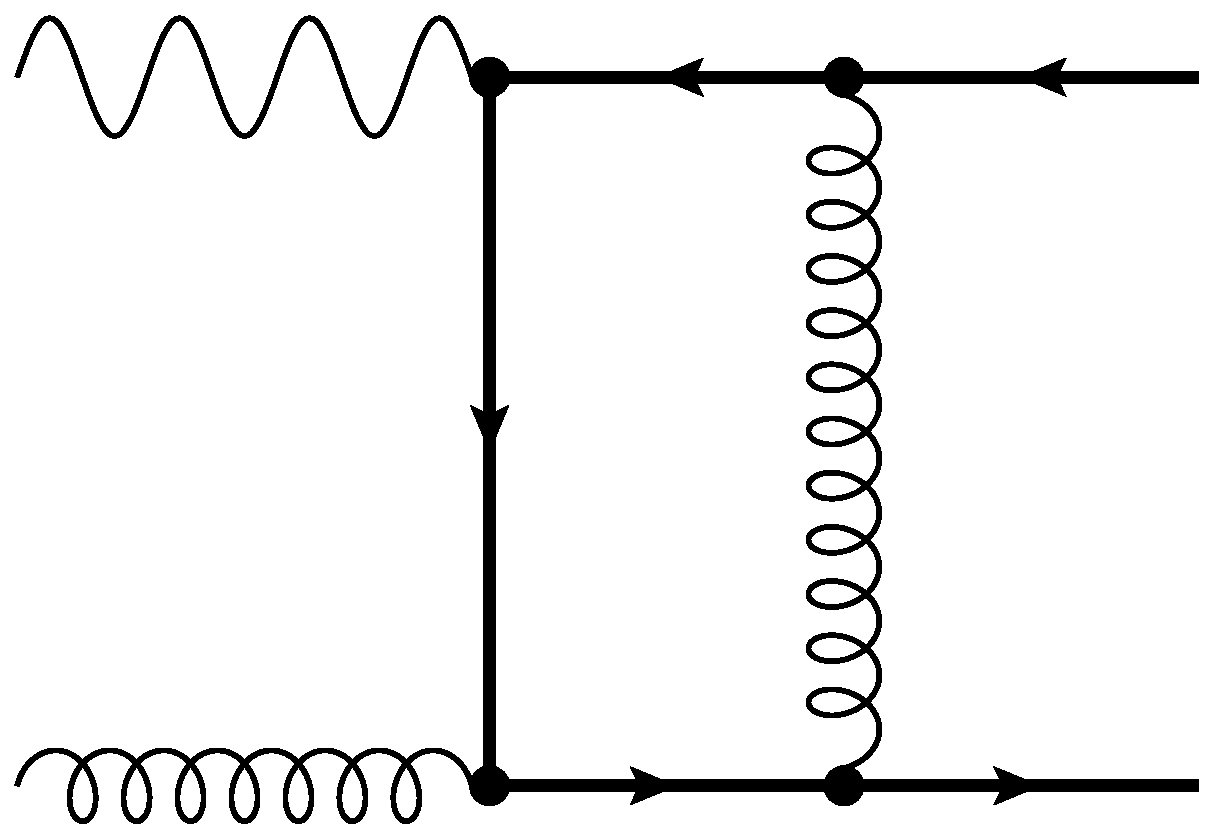
\includegraphics[height=.15\textheight]{img/nlo-v-1}} + %
\raisebox{-.4\height}{\includegraphics[width=.2\textwidth]{pyfeyn2/nlo-q-4}} + %
\raisebox{-.4\height}{\includegraphics[width=.2\textwidth]{pyfeyn2/nlo-q-3}} + \ldots
\item<3-> $\Rightarrow g_1 \sim e_u^2\cdot \Delta u \otimes d_{P,q}^{(1)}$
\item<3-> $d_{P,q}^{(1)}(\chi,\chi') = c_1(\chi,\chi')\ln(\chi) + c_2(\chi,\chi')\DiLog\left(\frac{1+\chi'}{1+\chi}\right)+\ldots$ \checkmark \iRef{Blümlein,Falcioni,De Freitas}
\item<3-> $\frac{m^2}{s} = \frac{\chi}{(1+\chi)^2}$ and $\frac{m^2}{s+Q^2} = \frac{m^2}{s'} = \frac{\chi'}{(1+\chi')^2}$ and $\frac{m^2}{Q^2} = \frac{\chi_q}{(1-\chi_q)^2}$
\item<4-> $\gamma_5$ and $\varepsilon_{\mu\nu\rho\sigma}$ in $n$-dimension? $\to$ HVBM scheme \iRef{'t Hooft,Veltman,Breitenlohner,Maison}
\end{itemize}
\end{frame}


\newcolumntype{w}{>{\centering\arraybackslash} m{.2\linewidth} }
\newcolumntype{n}{>{\centering\arraybackslash} m{.1\linewidth} }
\begin{frame}{Computation Review - Collinear Poles}
collinear poles appear in, e.g.,
\begin{center}
\begin{tabular}{wnw}
\includegraphics[width=.2\textwidth]{img/nlo-g-4}
&or
&\includegraphics[width=.2\textwidth]{img/nlo-q-1}
\end{tabular}
\end{center}

\begin{itemize}
\item remove by mass factorization $\to \MSbar$
\item $\Rightarrow g_1 \sim e_H^2\cdot \Delta g \otimes \ln(\mu_F^2/m^2) \bar c_{P,g}^{F,(1)}$
\item $\bar c_{P,g}^{F,(1)}(\chi,\chi_q) = c_1(\chi,\chi_q)\ln(\chi) + c_2(\chi,\chi_q)\DiLog\left(\frac{1-\chi_q}{1+\chi}\right) + \ldots$ (\checkmark for $Q^2\gg m^2$ \iRef{Buza,Matiounine,Smith,van Neerven})
\end{itemize}
\end{frame}

\begin{frame}{Computation Review - UV and IR Poles}
virtual diagrams are, e.g.,
\begin{center}
\begin{tabular}{wnw}
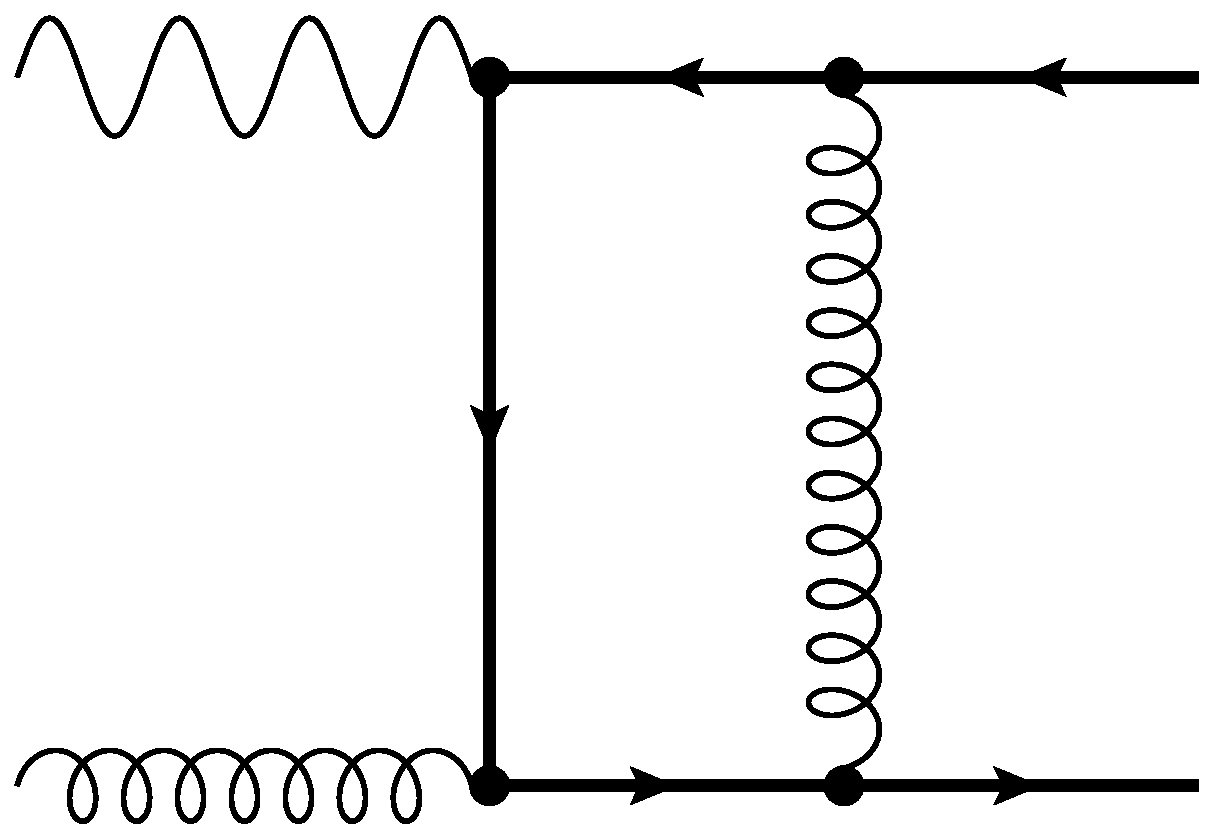
\includegraphics[width=.25\textwidth]{img/nlo-v-1}
&or
&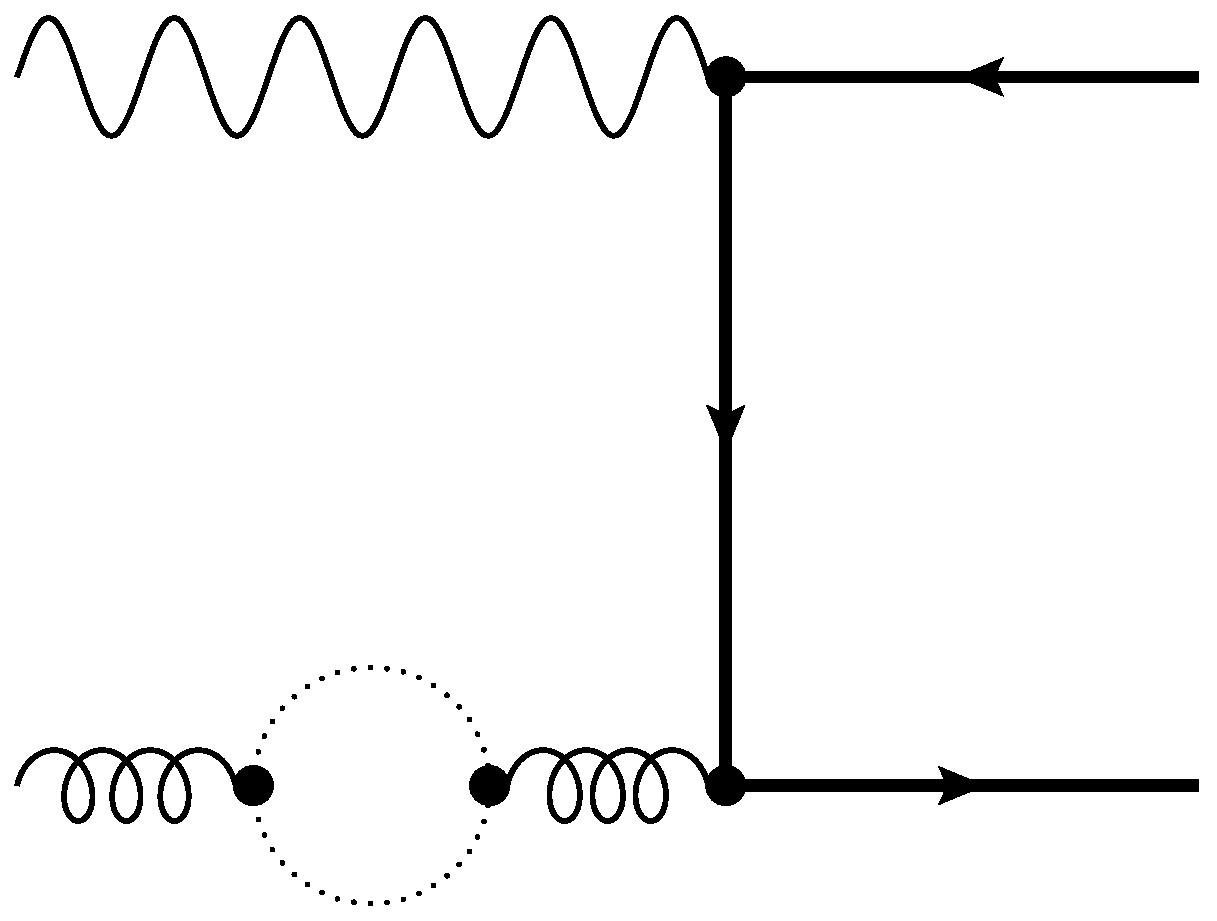
\includegraphics[width=.25\textwidth]{img/nlo-v-5}
\end{tabular}
\end{center}

soft poles appear in the limit of a soft gluon, e.g.,
\begin{center}
\includegraphics[width=.2\textwidth]{img/nlo-g-4}
\end{center}

soft + virtual + renormalization ($\MSbar_m$) + factorization is finite! \iRef{Laenen,Bojak}
\end{frame}

\begin{frame}[<+->]{Computation Review - Analytic Expressions}
\small
\begin{align*}
\nonumber
&D_0(m^2,0,q^2,m^2,t,s,0,m^2,m^2,m^2) = \frac{i C_\epsilon}{\beta s t_1}\times \Bigg[ -\frac{2}{\epsilon} \ln(\chi) -2\ln(\chi)\ln\left(\frac{-t_1}{m^2}\right)\\
\nonumber
&+\DiLog(1-\chi^2)-4\zeta(2)+\ln^2(\chi_q) + 2\DiLog(-\chi\chi_q)+2\DiLog\left(\frac{-\chi}{\chi_q}\right)\\
&+2\ln(\chi\chi_q) \ln(1+\chi\chi_q)+2\ln\left(\frac{\chi}{\chi_q}\right)\ln\left(1+\frac{\chi}{\chi_q}\right) \Bigg]
\end{align*}
\noindent\makebox[\linewidth]{\color{UniRot}\rule{\paperwidth}{0.4pt}}
\begin{align*}
\nonumber
\int\!\! \frac{d\Omega_n}{t' {u_7}^2} &= -\frac{2 \pi  (m^2+s_4) ({s'}+{t_1}) }{s_4 {t_1}^2 {u_1}^2} \Bigg[-2+\frac{{t_1} {u_1} (-q^2 s_4+(2 m^2+s_4) ({s'}+{u_1}))}{({s'}+{t_1}) \left(q^2 s_4 {t_1}+m^2 ({s'}+{u_1})^2\right)}\nonumber\\
 & +\frac{2}{\epsilon }+\ln\left(\frac{{t_1}^2 {u_1}^2 ({m^2}+{s_4})}{({s'}+{t_1})^2 \left({m^2} ({s'}+{u_1})^2+{q^2} {t_1} {s_4}\right)}\right)\Bigg]
\end{align*}\pause
\only<beamer:2->{\begin{textblock*}{5cm}(10cm,2cm) % {block width} (coords)
\includegraphics[width=5cm]{img/c1}
\end{textblock*}}
\end{frame}


\fxerror{write partonic}

\clearpage
\pagebreak


The hadronic reaction to study is deep-inelastic lepton-proton scattering:
\begin{equation}
\Pleptonminus(l_1) + \Pp(p) \rightarrow \Pleptonminus(l_2) + \PQ(p_1)(\PaQ(p_2)) + X
\end{equation}
where one either detects the heavy quark $\PQ$ \textit{or} the heavy anti quark $\PaQ$ and $X$ stands for any final hadronic state allowed by quantum-number conservation. We define then the hadronic Bjorken variables
\begin{equation}
q=l_1-l_2 \quad x=\frac{-q^2}{2p\cdot q} \quad z = \frac{p\cdot q}{p\cdot l_1}
\end{equation}

We can then define the measurable deep-inelastic hadron structure functions
\begin{align}
F_k(x,Q^2,m^2) &= \sum_{n=0}^\infty F_{k}^{(n)}(x,Q^2,m^2)\\
F_{k}^{(n)}(x,Q^2,m^2) &= \sum_{j\in\{\Pg,\Pq,\Paq\}}\int\limits_x^{z_{max}} \frac{dz}{z} f_j(x/z,\mu_F^2) \frac{-q^2}{4\pi^2\alpha} \sigma^{(n)}_{k,j}(s,q^2,m^2)
\end{align}
where $k\in\{G,L,P\}$ denotes as usual projection, $z=Q^2/s'$, $z_{max} = Q^2/(4m^2+Q^2)$ and $f_j(x/z,\mu_F^2)$ denotes parton momentum density functions\cite{Martin:2009iq,PhysRevLett.113.012001}.
We can then split the contributions whether there is a gluon in the initial state $F_{k,g}$ or a (anti)quark $F_{k,q}$. In leading order we find:
\begin{align}
F_{k,g}^{(0)}(x,Q^2,m^2) &= \frac{\alpha_sQ^2}{4\pi^2m^2}e_H^2\int\limits_x^{z_{max}}\frac{dz}{z} f_g(x/z,\mu_F^2) c^{(0)}_{k,g}(\eta,\xi)
\end{align}
In next-to-leading order we find for the gluonic part:
\begin{align}
&F_{k,g}^{(1)}(x,Q^2,m^2) \nonumber\\
 &= \frac{\alpha_s^2Q^2}{\pi m^2}e_H^2\int\limits_x^{z_{max}}\frac{dz}{z} f_g(x/z,\mu_F^2) \left(c_{k,g}^{(1)}(\eta,\xi) + \ln(\mu_F^2/m^2)\bar c_{k,g}^{F,(1)}(\eta,\xi) + \ln(\mu_R^2/m^2)\bar c_{k,g}^{R,(1)}(\eta,\xi)\right)
\end{align}
In next-to-leading order we find for the quark part:
\begin{align}
&F_{k,q}^{(1)}(x,Q^2,m^2) \nonumber\\
 &= \frac{\alpha_s^2Q^2}{\pi m^2}e_H^2\int\limits_x^{z_{max}}\frac{dz}{z} \left(\sum_{j=1}^{n_{lf}}f_{q(j)}(x/z,\mu_F^2)+f_{q(-j)}(x/z,\mu_F^2)\right) \nonumber\\
 &\hspace{120pt} \cdot\left(c_{k,q}^{(1)}(\eta,\xi) + \ln(\mu_F^2/m^2)\bar c_{k,q}^{F,(1)}(\eta,\xi)\right) \nonumber\\
 &\hspace{20pt} + \frac{\alpha_s^2Q^2}{\pi m^2}\int\limits_x^{z_{max}}\frac{dz}{z} \left(\sum_{j=1}^{n_{lf}}e_{q(j)}^2\left(f_{q(j)}(x/z,\mu_F^2)+f_{q(-j)}(x/z,\mu_F^2)\right)\right) d_{k,q}(\eta,\xi)
\end{align}
where we used the PDG particle labeling\cite{Hagiwara:2002fs}: $q(1)=u,q(-1)=\bar u,q(2)=d,q(-2)=\bar d$, \ldots and $e_u = e_c = e_t = 2/3, e_d=e_s=e_b=-1/3$. 

We can then also define some more practical functions:
\begin{align}
F_{2}(x,Q^2,m^2) &= F_{T}(x,Q^2,m^2) + F_{L}(x,Q^2,m^2)\\
 &= F_{G}(x,Q^2,m^2) + \frac 3 2 F_{L}(x,Q^2,m^2)\\
F_1(x,Q^2,m^2) &= (F_{2}(x,Q^2,m^2)-F_L(x,Q^2,m^2))/(2x)\\
 &= \left(F_{G}(x,Q^2,m^2)+\frac 1 2 F_{L}(x,Q^2,m^2)\right)/(2x)\\
g_1(x,Q^2,m^2) &= F_{P}(x,Q^2,m^2)/(2x)
\end{align}
and we define the spin asymmetry
\begin{align}
A_1(x,Q^2,m^2) &= \frac{g_1(x,Q^2,m^2)}{F_1(x,Q^2,m^2)} = \frac{F_P(x,Q^2,m^2)}{F_2(x,Q^2,m^2)-F_L(x,Q^2,m^2)}
\end{align}

For the plots we focused on charm production ($n_{lf}=3$) with $m_c=\SI{1.5}{\GeV}$ and we used the running coupling of \fxerror{cite,do}: We set $\mu_F^2=\mu_R^2=4m^2-q^2$ in analogy to \cite{Laenen1993162}.We used the PDF set MSTW2008nlo90cl\cite{Martin:2009iq,Martin:2009bu,Martin:2010db} provided by LHAPDF\cite{LHAPDF6} for the unpolarized structure functions ($F_2,F_G,F_L$) and DSSV2014\cite{PhysRevLett.113.012001} for the polarized structure function ($F_G$).

\fxerror{shift to appendix?}

\pagebreak
\begin{figure}[ht!]
\centering
\begin{subfigure}[t]{\textwidth}
	\input{img/F0012}
\end{subfigure}\\%
\begin{subfigure}[t]{\textwidth}
	\input{img/F001L}
\end{subfigure}\\%
\begin{subfigure}[t]{\textwidth}
	\input{img/F001P}
\end{subfigure}
\caption{hadronic structure functions $F_{k}(x,Q^2,m_c^2)$ plotted as function of $x$ for different values of $Q^2$ in units of $\si{\GeV^2}$}\label{fig:F001}
\end{figure}

\clearpage
\pagebreak


\section{Outlook}
\begin{frame}{Outlook}
\begin{itemize}
\item inclusive distributions: $\DeriveF{{p_{T,\PaQ}}}{g_1},\DeriveF{{y_{\PaQ}}}{g_1}$
\item correlated distributions: $\DeriveF{{M_{\PQ\PaQ}^2}}{g_1}, \DeriveF{\phi_{\PQ\PaQ}}{g_1}$
\item full neutral current (NC) contributions: $F_3^{\PZ\Pgg}, g_4^{\PZ\Pgg}, g_5^{\PZ\Pgg}$ and $F_2^{\PZ}, F_L^{\PZ}, g_1^{\PZ}$
\item distributions of full NC structure functions: $\DeriveF{p_{T,\PaQ}}{g_1^{NC}},\DeriveF{{M_{\PQ\PaQ}^2}}{g_1^{NC}}$
\end{itemize}

\vspace{1cm}
\setbeamercolor{thanks}{bg=UniRot,fg=white}
\begin{beamercolorbox}[ht=2.5ex,dp=1ex,center]{thanks}
Thank you for your attention!
\end{beamercolorbox}
\end{frame}


\end{document}
